In diesem Kapitel sollen die Anforderungen und Akzeptanztests für einen
Prototypen definiert werden. Als Grundlage sollen die Komponenten und
Verhaltensmuster der Applikation Strukti Live 1.2 dienen, da die Applikation
öffentlich verfügbar ist.

Wie im Kapitel \ref{chapter:MethodenZurEntscheidungsfindungBeiEinerEvaluation}
(\nameref{chapter:MethodenZurEntscheidungsfindungBeiEinerEvaluation}, S.
\pageref{chapter:MethodenZurEntscheidungsfindungBeiEinerEvaluation}ff)
beschrieben, gilt der Proof of Concept als erfolgreich, wenn alle
Akzeptanztests erfolgreich abgenommen wurden. Die Abnahme der Akzeptanztests
erfolgt durch eine visuelle Prüfung.

\section{Anforderungen mit User Stories}

\begin{description}
\item[US-1\label{itm:US-1}]
Es soll das Fenster in sechs Teile (Panels) aufgeteilt werden. Die Aufteilung
soll in drei Spalten und zwei Zeilen aufgeteilt werden, wobei die erste Zeile
eine Höhe von 150px\footnote{px ist die Abkürzung für Pixel, zu Deutsch
Bildpunkt. Ein Pixel bezeichnet die kleinste Einheit einer digitalen
Rastergrafik.} und die zweite Zeile eine höhe von 606px haben soll.

\item[US-2\label{itm:US-2}]
Es soll die erste und die dritte Spalte eine Breite von 220px und die zweite
und mittlere Spalte eine Breite von 552px haben.

\item[US-3\label{itm:US-3}]
Es soll der Panel in der ersten Zeile und der ersten Spalte immer ein Logo der
Applikation dargestellt werden. Wenn mit der linken Maustaste auf das Bild
``geklickt'' wird, soll die Startansicht geladen werden.

\item[US-4\label{itm:US-4}]
Es soll der Panel in der ersten Zeile und der zweiten Spalte der Hintergrund
hellblau eingefärbt werden. In der linken unteren Ecke des Panels soll der Titel
der aktuellen Ansicht angezeigt werden.

\item[US-5\label{itm:US-5}]
Es soll der Panel in der zweiten Zeile und der ersten Spalte als
Navigationspanel dienen. Die verschiedenen Ansichten sollen über den
Navigationspanel angesteuert werden können.

\item[US-6\label{itm:US-6}]
Der Navigationspanel soll eine zweistufige Navigation anbieten. Ansichten,
welche Gruppiert werden können, sollen in der zweiten Stufe untergebracht
werden. Navigationen, welche sich in der zweiten Stufe befinden, sollen
unterhalb der übergeordneten Navigationen eingeruckt dargestellt werden.

\item[US-7\label{itm:US-7}]
Die aktuell angesteuerte Ansicht soll im Navigationspanel andersfarbig
dargestellt werden.

\item[US-8\label{itm:US-8}]
Im Navigationspanel sollen die verschiednen Navigationspunkte auf der ersten
Stufe über ein Separator visuell voneinander getrennt werden.

\item[US-9\label{itm:US-9}]
Wenn ein Navigationspunkt der ersten Stufe im Navigationspanel ``angeklickt''
wird, sollen die darunter liegenden zweitstufigen Navigationspunkt sichtbar
werden.

\item[US-10\label{itm:US-10}]
Es sollen zwei Navigationen auf der ersten Stufen angezeigt werden. Die
Navigationen sind ``Einführung'' und ``Produktauswahl''.

\item[US-11\label{itm:US-11}]
Es sollen zwei Navigationen auf der zweiten Stufen unterhalb der Navigation
``Produktauswahl'' angezeigt werden. Die Navigationen sind
``Produktbeschreibung'' und ``Produktdesign''.

\item[US-12\label{itm:US-12}]
Wenn der Navigationspunkt ``Einführung'' ausgewählt wird, soll in der zweiten
Reihe und der zweiten Spalte ein Einführungstext zum Proof of Concept
dargestellt werden.

\item[US-13\label{itm:US-13}]
Wenn der Navigationspunkt ``Produktauswahl'' ausgewählt wird, soll in der
zweiten Reihe und der zweiten Spalte eine Buttonmatrix mit den Produkten
``Put Option'', ``Soft Runner'' und ``Protein'' dargestellt werden. Die
Navigationen ``Produktbeschreibung'' und ``Produktdesign'' sollen angezeigt
werden und deaktiviert sein.

\item[US-14\label{itm:US-14}]
Wenn der Navigationspunkt ``Produktauswahl'' ausgewählt wird, sollen in der
zweiten Zeile und der dritten Spalte Filteroptionen für die Produkte in der Form
von CheckBoxen dargestellt werden.

\item[US-15\label{itm:US-15}]
Wenn eine Filteroption gewählt wird, sollen die Produkte entsprechend des
Filters aktiv oder inaktiv gesetzt werden.

\item[US-16\label{itm:US-16}]
Wenn ein Produkt ausgewählt wird, dann soll in der zweiten Reihe und der zweiten
Spalte die Produktbeschreibung angezeigt werden. Die Produktbeschreibung
besteht aus einem Fliesstext und einem TabbedPanel welcher sechs Tabs hat:
``Eigenschaften'', ``Chancen \& Risiken'', ``Rückzahlungsmodus'',
``Beispiele'', ``Steuern'' und ``Klassifizierung''. Die Navigationspunkte
``Produktbeschreibung'' und ``Produktdesign'' sollen nun aktiv gesetzt werden.

\item[US-17\label{itm:US-17}]
Wenn ein Tab ausgewählt wird, sollen die entsprechenden Informationen zum
Produkt dargestellt werden.

\item[US-18\label{itm:US-18}]
Wenn der Navigationspunkt ``Produktdesign'' ausgewählt wird, soll das
Auszahlungsprofil eines möglichen Produkts dargestellt werden. Die notwendigen
Eckdaten sollen in der zweiten Zeile und der dritten Spalte in der Form von
Slidern dargestellt werden.

\item[US-19\label{itm:US-19}]
Wenn die Werte in den Slidern geändert werden, dann soll sich das
Auszahlungsprofil entsprechend anpassen.
\end{description}

\section{Priorisierung der User Stories}

Es wurden alle 19 User Stories als \begin{itshape}hoch\end{itshape} priorisiert.

\section{Akzeptanztests}

Für alle Akzeptanztests gilt als Voraussetzung, dass der Prototyp auf einem
Applikationsserver läuft. Die Akzeptanztest werden mit den Webbrowsern Chrome,
Safari und Firefox durchgeführt, um sicherzustellen dass der Prototyp unabhängig
vom Webbrowser implementiert wurde.

Firefox wird in der \ac{ZKB} offiziell als Browser unterstützt, desshalb wurde
er als Testkandidat miteinbezogen. Chrome und Safari sind die beiden Browsern
welche in diesem Jahr am meisten Marktanteile dazugewonnen haben, siehe
\cite{BrowserStatistik}. Aus diesem Grund wurden sie als Testkandidaten gewählt.

\begin{description}
\item[T-1.1\label{itm:T-1.1}]
Die vorgegebenen Masseinheiten der Zeilen sollen mit einem Screenshot geprüft werden.

\item[T-2.1\label{itm:T-2.1}]
Die vorgegebenen Masseinheiten der Spalten sollen mit einem Screenshot geprüft werden.

\item[T-3.1\label{itm:T-3.1}]
Es soll geprüft werden, ob das Logo in der ersten Zeile und der ersten Spalte
vorhanden ist.

\item[T-3.2\label{itm:T-3.2}]
Mit einem Klick auf das Logo soll die Startansicht geladen werden.

\item[T-4.1\label{itm:T-4.1}]
Es soll geprüft werden, ob der Panel in der ersten Zeile und der zweiten Spalte
einen hellblau eingefärbten Hintergrund hat.

\item[T-4.2\label{itm:T-4.2}]
Durch das navigieren über verschiedene Menüpunkte, soll der Titel in der ersten
Zeile und der zweiten Spalte, entsprechend der aktuellen Ansicht, angepasst
werden.

\item[T-5.1\label{itm:T-5.1}]
Es soll geprüft werden, ob die Navigation in der zweiten Zeile und der
ersten Spalte ersichtlich ist.

\item[T-5.2\label{itm:T-5.2}]
Durch das navigieren über verschiedene Menüpunkte, soll sich entsprechend die
Ansicht ändern.

\item[T-6.1\label{itm:T-6.1}]
Es soll geprüft werden, ob gruppierte Navigationen unterhalb, der von ihnen
übergeordnenten Navigation, eingeruckt dargestellt werden.

\item[T-7.1\label{itm:T-7.1}]
Es soll geprüft werden, ob die Farbe sich bei einer angesteuerten Navigation
ändert.

\item[T-8.1\label{itm:T-8.1}]
Es soll geprüft werden, ob die Navigationspunkt auf der ersten Stufe über ein
Separator voneinander getrennt sind.

\item[T-8.2\label{itm:T-8.2}]
Wenn ein Navigationspunkt der ersten Stufe angewählt wird, unter der sich
Navigationspunkte auf der zweiten Stufe befinden, soll überprüft werden, dass
kein Separator zwischen der ersten und der zweiten Stufe existiert.

\item[T-9.1\label{itm:T-9.1}]
Wenn ein Navigationspunkt der ersten Stufe angewählt wird, unter der sich
Navigationspunkte auf der zweiten Stufe befinden, soll überprüft werden, ob
diese angezeigt werden.

\item[T-10.1\label{itm:T-10.1}]
Die beiden Navigationspunkte ``Einführung'' und ``Produktauswahl'' sollen auf
der ersten Stufe angezeigt werden.

\item[T-11.1\label{itm:T-11.1}]
Wenn der Navigationspunkt ``Produktauswahl'' angewählt wurde, sollen die beiden
Navigationspunkt ``Produktbeschreibung'' und ``Produktdesign'' auf der zweiten
Stufe angezeigt werden.

\item[T-12.1\label{itm:T-12.1}]
Wenn der Navigationspunkt ``Einführung'' angewählt wurde, soll in der zweiten
Zeile und der zweiten Spalte ein Einführungstext zum Proof of Concept
dargestellt werden.

\item[T-13.1\label{itm:T-13.1}]
Wenn der Navigationspunkt ``Einführung'' angewählt wurde, soll in der zweiten
Reihe und der zweiten Spalte eine Buttonmatrix mit den möglichen Produkten
angezeigt werden.

\item[T-13.2\label{itm:T-13.2}]
Die Navigationspunkte ``Produktbeschreibung'' und ``Produktdesign'' sollen
deaktiviert sein.

\item[T-14.1\label{itm:T-14.1}]
Es soll geprüft werden, ob die Filteroptionen in der zweiten Reihe und der
dritten Spalte dargestellt werden, wenn der Navigationspunkt ``Produktauswahl''
angewählt wurde.

\item[T-14.2\label{itm:T-14.2}]
Die Filteroptionen sollen in der Form von CheckBoxen angezeigt werden.

\item[T-15.1\label{itm:T-15.1}]
Es soll eine Filteroption ausgewählt werden, dabei sollen sich die Produkte,
welche durch den Filter ausgeschlossen werden, deaktiviert werden.

\item[T-15.2\label{itm:T-15.2}]
Es soll eine Filteroption, welche ausgewählt war, wieder abgewählt werden. Dabei
sollen sich die Produkte, welche durch den Filter ausgeschlossen waren, wieder
aktiviert werden.

\item[T-16.1\label{itm:T-16.1}]
Es soll ein Produkt gewählt werden. Wenn das Produkt ausgewählt wurde, soll in
der zweiten Reihe und der zweiten Spalte die Produktbeschreibung angezeigt
werden.

\item[T-16.2\label{itm:T-16.2}]
Die Produktbeschreibung soll aus einem Fliesstext und einem TabbedPanel
bestehen.

\item[T-16.3\label{itm:T-16.3}]
Wenn die Produktbeschreibung angezeigt wird, sollen sechs Tabs angezeigt
werden: ``Eigenschaften'', ``Chancen \& Risiken'', ``Rückzahlungsmodus'',
``Beispiele'', ``Steuern'' und ``Klassifizierung''.

\item[T-16.4\label{itm:T-16.4}]
Wenn ein Produkt ausgewählt wurde, sollen die Navigationspunkte
``Produktbeschreibung'' und ``Produktdesign'' aktiv gesetzt werden.

\item[T-17.1\label{itm:T-17.1}]
Wenn das Produkt ``Put Option'' ausgewählt wird, sollen die Informationen in den
Tabs angezeigt werden.

\item[T-18.1\label{img:T-18.1}]
Wenn das Produkt ``Put Option'' ausgewählt wird, und danach der Navigationspunkt
``Produktdesign'' angewählt wird, soll das Auszahlungsprofil einer Put Option
angezeigt werden.

\item[T-18.2\label{img:T-18.2}]
Wenn der Navigationspunkt ``Produktdesign'' angewählt wird, soll in der zweiten
Zeile und der dritten Spalte der Strike und die Volatilität mit einem Slider
angepasst werden können.

\item[T-19.1\label{img:T-19.1}]
Wenn die Werte der Slider geändert werden, soll das Auszahlungsprofil
entsprechend angepasst werden.
\end{description}

\section{Testabdeckung}

Die Testabdeckung ist in der Tabelle \ref{tab:testabdeckung} ersichtlich und
beträgt 100\%. Somit gilt der Proof of Concept, gemäss dem Kapitel
\ref{chapter:MethodenZurEntscheidungsfindungBeiEinerEvaluation}
(\nameref{chapter:MethodenZurEntscheidungsfindungBeiEinerEvaluation}, S.
\pageref{chapter:MethodenZurEntscheidungsfindungBeiEinerEvaluation}ff), als
erfolgreich.

\begin{table}[h!]
  \sffamily 
  \begin{center}
    \begin{tabular}{llrr}
      \toprule
      \textbf{Browser} & \textbf{Version} & \textbf{Testfälle durchgeführt} &
      \textbf{Erfolgreich}\\
      \midrule
      Chrome & 12.0.742.91 & 30 & 100\% \\
      Safari & 5.0.5 (6533.21.1) & 30 & 100\% \\
      Firefox & 4.0.1 & 30 & 100\% \\
      \bottomrule
    \end{tabular}
    \caption{Testabdeckung der Testfälle für den Proof of Concept}
    \label{tab:testabdeckung}
  \end{center}
\end{table}

\section{Resultat}

In einem Proof of Concept konnte gezeigt werden, dass Vaadin den Anforderungen
an ein Java Web Framework entspricht.

Die Art und Weise wie man in Vaadin programmiert, entspricht ziemlich genau
dem Programmierstil von Java Swing. Es werden äquivalente Typen von Komponenten
und Layoutmanagern angeboten, die Kommunikation zwischen den Komponenten
wird über das Observer Design Pattern implementiert. Zudem biete Vaadin eigene
Themes an, welche beliebig erweitert werden können, ähnlich dem pluggable Look
\& Feel von Java Swing. Leider kommt man dabei nicht ganz ohne \ac{CSS} aus, was
den Erwartungen entsprochen hätte.

In den Abbildungen \ref{img:poc1}, \ref{img:poc2} und \ref{img:poc3} ist das
Resultat in Form vom Screenshots ersichtlich. Es werden dabei drei
verschiedene Ansichten mit erkannten Swingkomponenten gezeigt.
\newline

\begin{figure}[htb]
  \begin{center}
    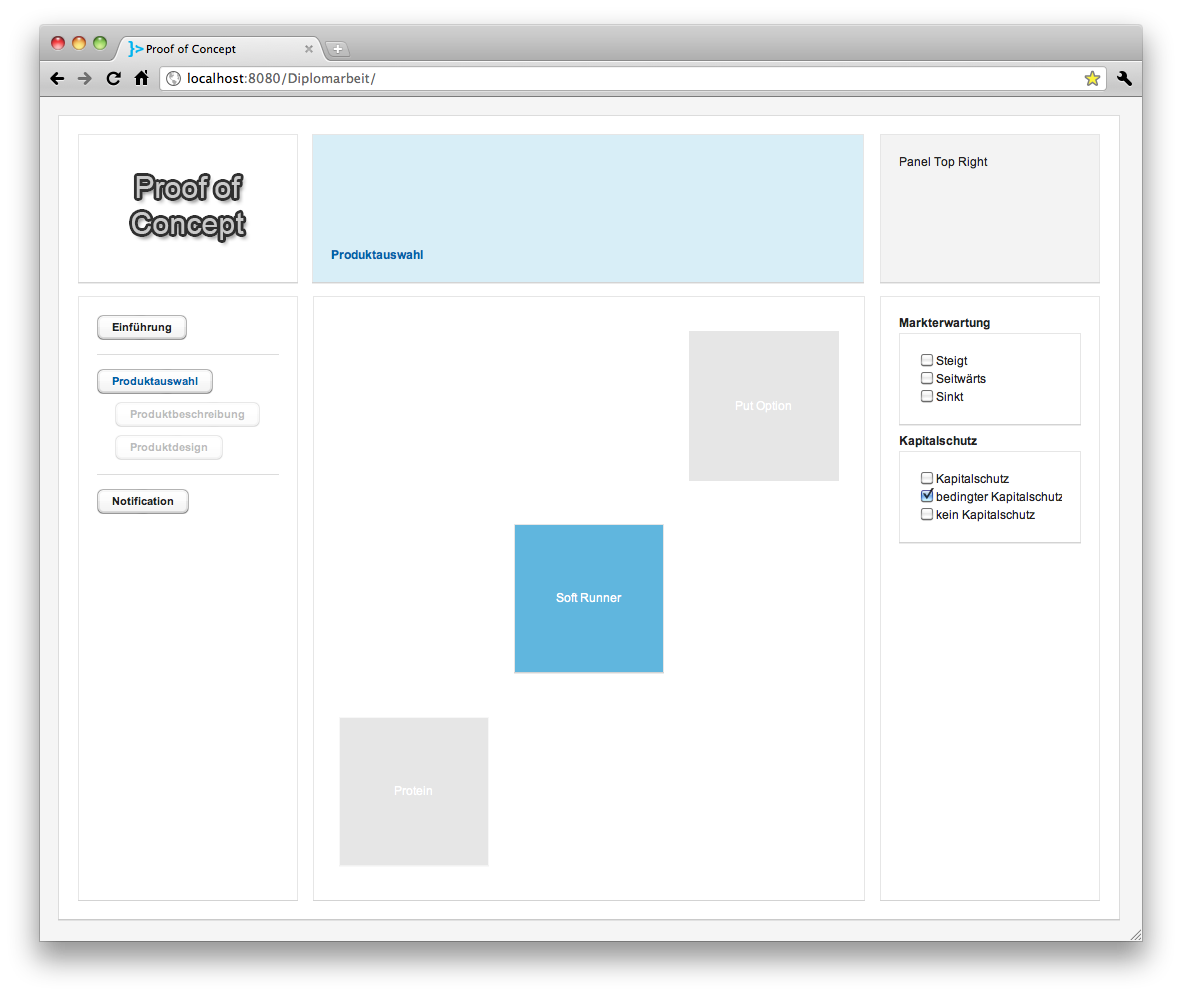
\includegraphics[width=0.7\textwidth]{./image/POC/poc1.png}
    \caption{Ansicht der Produkt in der Form einer Button Matrix.}
    \label{img:poc1}
  \end{center}
\end{figure}

\begin{figure}[htb]
  \begin{center}
    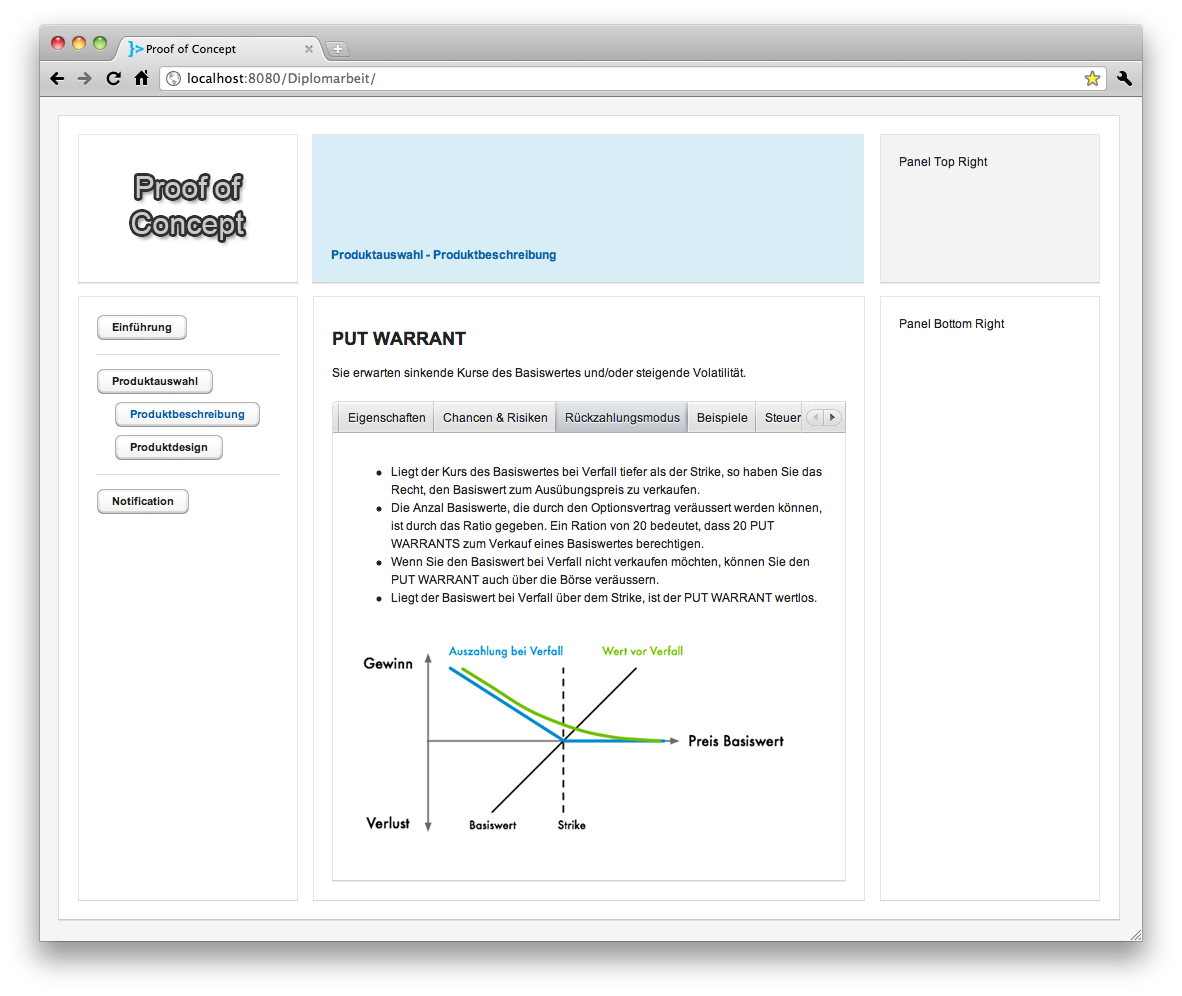
\includegraphics[width=0.7\textwidth]{./image/POC/poc2.png}
    \caption{Produktbeschreibung einer Put Option mit einem Tabbed Panel.}
    \label{img:poc2}
  \end{center}
\end{figure}

\begin{figure}[htb]
  \begin{center}
    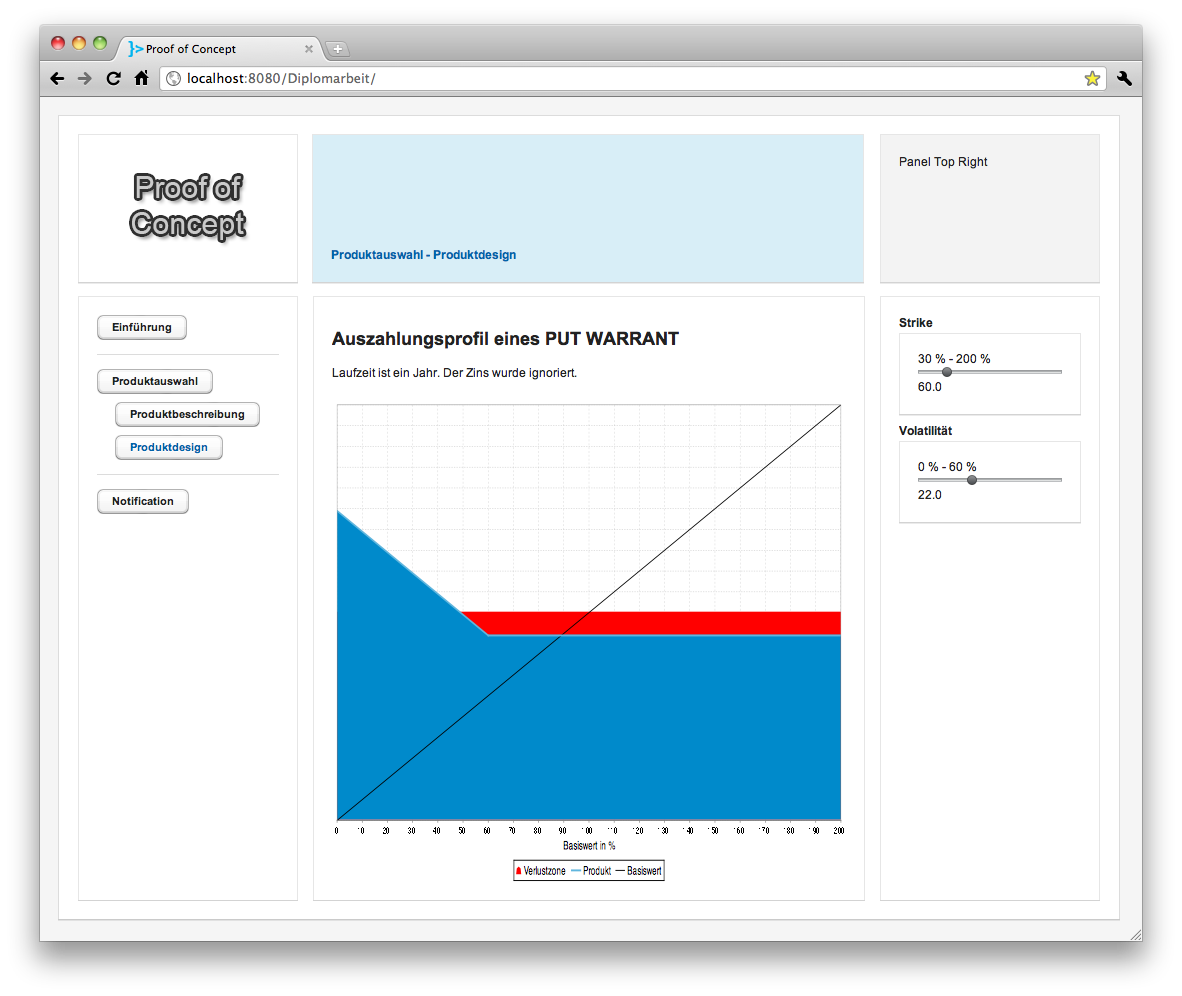
\includegraphics[width=0.7\textwidth]{./image/POC/poc3.png}
    \caption{Ansicht eines Auszahlungsprofils einer Put Option mit einem
    JFreeChart.}
    \label{img:poc3}
  \end{center}
\end{figure}

Der Sourcecode des Proof of Concept ist bei GitHub\footnote{GitHub ist ein
webbasierter Hosting-Dienst für Software-Entwicklungsprojekte.} öffentlich
zugänglich unter der URL \url{https://github.com/sushicutta/Diplomarbeit}. Das
Projekt ist für die \ac{IDE} Eclipse\footnote{Eclipse ist ein quelloffenes
Programmierwerkzeug zur Entwicklung von Software verschiedenster Art.}
aufgesetzt. Eclipse ist unter der URL
\url{http://www.eclipse.org/downloads/} kostenlos erhältlich. Für den Betrieb
wird das Eclipse GlassFish\footnote{GlassFish ist ein Open-Source-Projekt eines
Java EE Servers von Oracle} Plug-in benötigt, welches sich um das Deployment
der Applikation und den Betrieb des Applikationensserver kümmert. Das Plug-in
ist unter der URL \url{http://glassfishplugins.java.net/} kostenlos erhältlich.
